\section{Обзор}
В данном разделе представлен обзор предметной области:
основные способы реализации предметно-ориентированных языков; 
процесс отображения пользовательских интерфейсов;
существующие языки программирования общего назначения, предоставляющие
пользователям возможность декларативного описания пользовательских
интерфейсов с помощью предметно-ориентированных языков.

\subsection{Предметная область}
\subsubsection{Предметно-ориентированные языки}
\label{dsl-section}
Предметно-ориентированный язык (\textit{domain-specific language}, DSL) ---
это язык программирования с более высоким уровнем абстракции,
отражающий специфику решаемых с его помощью задач. Такой язык оперирует
понятиями и правилами из определенной предметной области~\cite{book-of-dsls}.

В отличие от языков программирования общего назначения, таких как \name{C},
\name{Python}, \name{Java}, предметно-ориентированные языки предоставляют
абстракции, адекватные решаемой проблеме, позволяя выражать решения,
написанные с их помощью, кратко и ёмко; причём в некоторых случаях
использование DSL не требует квалификации программиста.
В качестве примера DSL можно привести \name{SQL} ---  декларативный язык
программирования, применяемый для создания, модификации и управления данными в
реляционной базе данных.
Основным недостатком применения предметно-ориентированных языков является
стоимость их разработки, требующая экспертизы как в области разработки языков
программирования, так и в целевой предметной области.
Это является одной из причин того, что предметные языки редко применяются
для решения задач программной инженерии, в отличие от языков программирования
общего назначения.
Другой причиной отказа от обособленных предметных языков является тот факт,
что сочетание программной библиотеки и языка программирования общего
назначения может заменять DSL.
Программный интерфейс (\textit{Application Programming Interface},
API) библиотеки содержит специфичный для определённой
области словарь, образованный именами классов, методов и функций, доступный
всем пользователям языков программирования общего назначения, подключившим
библиотеку.
Однако, вышеприведённый подход проигрывает предметным языкам в следующих
аспектах~\cite{when-and-how-develop-dsl,dsl-spectrum-wile}:
\begin{itemize}
	\item устоявшаяся в области нотация, как правило, выходит за рамки
	ограниченных механизмов определения пользовательских операторов,
	предоставляемых языками общего назначения;
	\item абстракции определённой области не всегда могут быть
	просто отображены в конструкции языков общего назначения~\cite{dsl-traversal-transform};
	\item использование предметно-ориентированного языка сохраняет
	возможность анализа, верификации, оптимизации, параллелизации и
	трансформации в рамках конкретной области, что, в случае работы с
	исходным текстом языка программирования общего назначения, является
	более сложной задачей.
\end{itemize}

\subsubsection{Подходы к реализации предметно-ориентированных языков}
В последнее время всё больше исследований в области
предметно-ориен\-тированных языков направлены на категоризацию предметных
языков, а также выработку советов и лучших практик, отвечающих на вопросы
"когда и как?" создавать DSL для конкретной области~\cite{when-and-how-develop-dsl,study-on-preliminary-approaches-develop-dsl,spinellis-dsl-patterns}.
\paragraph{Препроцессинг}
DSL-конструкции транслируются в более низкоуровневый программный код
базового языка программирования общего назначения.
\begin{itemize}
	\item \textit{Макрокоманда}. Конструкции предметного языка представлены
	символьными именами, заменяемыми при обработке препроцессором на
	последовательность программных инструкций базового языка.
	\item \textit{Транспиляция}. Исходный код предметного языка
	транслируется в исходный код языка общего назначения.
	\item \textit{Лексическая обработка}. Трансформация предметного языка в
	язык общего назначения осуществляется на уровне лексем.
\end{itemize}

Преимуществом данного подхода является простота реализации DSL, поскольку
большая часть семантического анализа выполняется средствами базового языка.
В то же время, это является и недостатком данного подхода ввиду отсутствия
предметно-ориентированного статического анализа, оптимизаций и сообщений об ошибках.

\paragraph{Встраивание в базовый язык}
В данном подходе конструкции базового языка используются для построения
библиотеки предметно-ориен\-тированных операций. С помощью синтаксиса
базового языка задаётся диалект, максимально приближенный к определённой
предметной области.

Преимуществом данного подхода является полное переиспользование компилятора или интерпретатора базового языка для построения DSL. Основными недостатками
являются сообщения об ошибках, соответствующие спецификации базового языка,
и ограниченная синтаксическая выразительность, обусловленная
существующим синтаксисом базового языка.

\paragraph{Самостоятельный компилятор}
В данном подходе для создания DSL используются методы построения
компиляторов или интерпретаторов. В случае компилятора, конструкции
предметного языка транслируются во внутреннее представление компилятора, а
статический анализ производится над спецификацией DSL. В случае
интерпретатора, конструкции предметного языка распознаются и выполняются
в ходе цикла выборки-распознавания-исполнения (fetch-decode-execute cycle).

Преимуществами данного подхода являются приближенные к предметной
области синтаксис языка и сообщения об ошибках. Серьёзным недостатком
является необходимость создания нового компилятора или интерпретатора
предметного языка.

\paragraph{Компилятор компиляторов}
Данный подход схож с предыдущим за исключением того, что все или некоторые
стадии компиляции выполняются с использованием \textit{компилятора компиляторов} --- программы, воспринимающей синтаксическое или семантическое
описание языка программирования и генерирующей компилятор для этого языка.

Преимуществом подхода является снижение расходов на создание компилятора
предметного языка. Ограниченность итогового DSL возможностями используемого
компилятора компиляторов, а также сложность проработки предметного языка в
деталях, что может быть критично для достижения определённого уровня
производительности и близости сообщений об ошибках к предметной области,
составляют недостатки данного подхода.

\paragraph{Расширение существующего компилятора}
Компилятор языка программирования общего назначения расширяется
предметно-ориенти\-рованными правилами оптимизации и/или генерации кода.

В сравнении с предыдущим, данный подход менее трудоёмок из-за возможности
переиспользования частей существующего компилятора. Однако, стоит отметить,
что расширение существующего компилятора может оказаться сложной задачей,
для выполнения которой необходима поддержка расширений со стороны
компилятора языка общего назначения, а также минимизация пересечений
синтаксиса и семантики базового и предметного языков.

\paragraph{Использование готовых инструментов}
Существующие инструменты и нотации адаптируются под конкретную предметную
область. Примером такого подхода являются DSL, основанные на нотации
\name{XML}. В большинстве случаев предметные языки, полученные данным
способом, плохо подходят для их использования людьми в ручном режиме.

\newpage
\subsubsection{Отображение пользовательского интерфейса}
В данном разделе представлен один из способов
отображения пользовательских интерфейсов, использующийся в популярных
средствах разработки приложений~\cite{flutter-homepage,swift-homepage,
vuenative-homepage,reactnative-homepage}. Графическая подсистема
языка \name{Accord} основана на схожем подходе. Стоит также отметить, что
далее будут рассмотрены лишь базовые принципы построения и отображения
интерфейсов, которых должно быть достаточно для объяснения тех или иных
оптимизационных решений, принятых в данной работе.

Задачей построения и отображения пользовательского интерфейса занимается
так называемый движок рендеринга или отрисовки (\textit{ren\-dering engine})
--- программное обеспечение, получающее изображение по какой-либо модели.
Здесь \textit{модель} --- это описание любых объектов или явлений на строго
определённом языке или в виде структуры данных.

На рисунке~\ref{render-pipeline} представлен схематичный шаг алгоритма
рендеринга пользовательского интерфейса. Так, отрисовка кадра \textit{N}
состоит из нескольких последовательных этапов:
\begin{enumerate}
	\item построение дерева компонентов по текущему состоянию
	пользовательского интерфейса. \textit{Дерево компонентов} ---
	древовидная структура данных, элементами которой являются
	высокоуровневые компоненты интерфейса. Примером такого дерева
	может являться \name{DOM} (от англ. \textit{Document Object Model} ---
	объектная модель документа), использующийся в современных веб-браузерах.
	\item построение дерева элементов по дереву компонентов. \textit{Дерево
	элементов} --- древовидная структура данных, изоморфная дереву
	компонентов, элементами которой являются структуры данных движка
	рендеринга.
	\item построение дерева рендеринга по дереву элементов. \textit{Дерево
	рендеринга} --- древовидная структура данных, содержащая в себе только
	необходимые для непосредственно рендеринга элементы интерфейса. Говоря
	о переходе между деревом элементов и деревом рендеринга как об
	отображении, можно сказать, что не все узлы дерева элементов имеют
	свой образ в дереве рендеринга. Так же стоит отметить, что узлы дерева
	рендеринга содержат в себе низкоуровневую информацию, такую как
	относительные координаты элемента в виртуальном пространстве движка
	отрисовки.
	\item размещение и отрисовка: перевод всех относительных свойств
	элементов в абсолютные, например, перевод относительных координат
	элемента в виртуальном пространстве движка отрисовки в координаты
	элемента на экране реального устройства; формирование запроса к
	аппаратуре для отрисовки интерфейса.
\end{enumerate}

\begin{figure}[h]
\centering
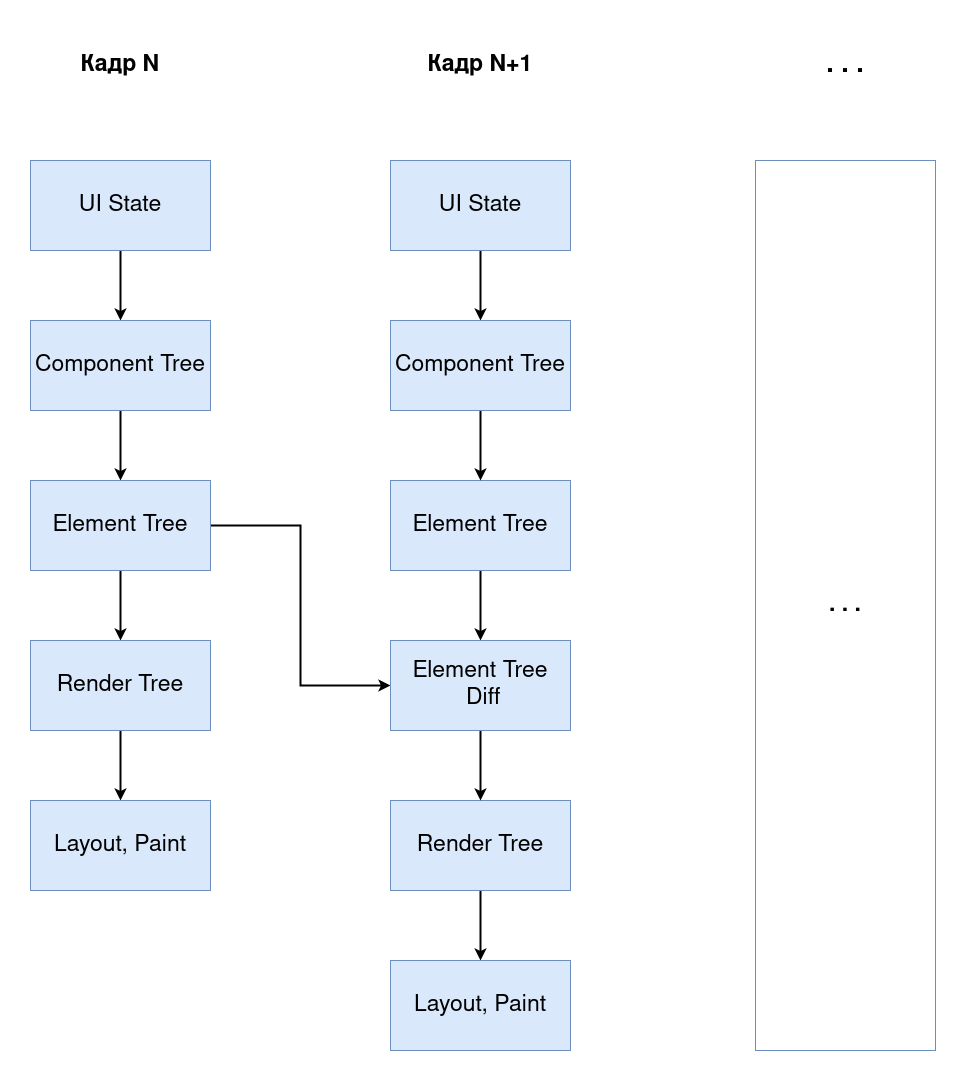
\includegraphics[width=\linewidth,height=0.9\linewidth,keepaspectratio]{resources/ui-render-pipeline.png}
\caption{Схематичный шаг алгоритма рендеринга пользовательского интерфейса}
\label{render-pipeline}
\end{figure}

Процесс отрисовки кадра \textit{N+1}, в свою очередь, повторяет
вышеописанный алгоритм за исключением следующего: дерево рендеринга
перестраивается на основании разницы между деревьями элементов текущего и
предыдущего кадров.
Подобное дополнение позволяет значительно повысить производительность
всего графического конвейера за счёт переиспользования вычислений,
хранящихся в дереве рендеринга предыдущего кадра.


\subsection{Существующие решения}
\subsubsection*{Dart/Flutter}
\name{Flutter}~\cite{flutter-homepage} --- язык разработки
мобильных приложений, разрабатываемый компанией \name{Google}. По
сравнению с остальными решениями, данный язык в меньшей степени является
предметно-ориентированным, поскольку реализован в виде библиотеки
графических компонентов, создающей словарь предметной области, для языка
программирования общего назначения \name{Dart}~\cite{dart-homepage}.

Графический интерфейс приложения на языке \name{Dart}/\name{Flutter}
описывается декларативно:
\begin{lstlisting}[language=Swift,caption=Счётчик нажатия кнопки на языке
\name{Dart}/\name{Flutter},label={lst:flutter-example}]
import '...'

class CounterApp extends StatelessWidget {
    @override
    Widget build(BuildContext context) {
        return MaterialApp(
            home: Counter(someCondition),
        );
    }
}

class Counter extends StatefulWidget {
    final bool condition;
    const Counter(this.condition);
    
    @override
    _CounterState createState() => _CounterState();
}

class _CounterState extends State<Counter> {
    int _counter = 0;
    
    void _incrementCounter() {
        setState(
            () { _counter++; }
        );
    }
    
    @override
    Widget build(BuildContext context) {
        return Column(
            children: <Widget>[
                Text("Current count: $_counter"),
                TextButton(
                    onPressed: _incrementCounter,
                    child: Text("Click on me!")
                ),
                widget.condition ?
                    Image.asset("assets/images/image.png") :
                    Text("Text Component")
            ]
        )
    }
}
\end{lstlisting}

\subsubsection*{Swift/SwiftUI}
\name{SwiftUI}~\cite{swiftui-homepage} --- язык разработки мобильных
приложений, разрабатываемый компанией \name{Apple}. Данный
предметно-ориентированный язык реализован методом встраивания в базовый
язык, которым, в данном случае, является язык программирования общего
назначения \name{Swift}~\cite{swift-homepage}. В отличие от языка
\name{Swift}, являющегося открытым и свободным программным обеспечением,
исходный код и спецификация \name{SwiftUI} являются проприетарными и
закрытыми, что не позволяет провести полноценный анализ данного решения.
При этом, на основе наблюдаемого поведения программ, написанных на языке
\name{SwiftUI}, и доступной документации можно сделать некоторые выводы о
реализации \name{SwiftUI}.

Графический интерфейс приложений на языке \name{SwiftUI}
описывается декларативно:
\begin{lstlisting}[language=Swift,caption=Счётчик нажатия кнопки на языке
\name{SwiftUI},label={lst:swiftui-example}]
struct ContentView : View {
    let condition: bool
    @State var count: Int = 0
	
    var body: some View {
        VStack {
            Text("Current count: \(count)")
            Button(action: {
                self.count += 1
            }) {
                Text("Click on me!")
            }
            if condition {
                Image("path/to/image")
            } else {
                Text("text component")
            }
        }
    }
}
\end{lstlisting}
Каждый компонент графического интерфейса, описываемый пользователем, должен
явно указывать на своё соответствие специальному протоколу (TODO: описание протоколов)
\name{View}. Согласно этому протоколу, тип, соответствующий ему, обязан
иметь поле \name{body} типа, также соответствующего протоколу \name{View}.
На языке \name{Swift} данный протокол может быть описать следующим образом:
\begin{lstlisting}[language=Swift, caption=Реализация протокола \name{View}
на языке \name{Swift}]
protocol View {
    associatedtype Body: View
    var body: Self.Body { get }
}
\end{lstlisting}

Для достижения декларативности, представленной на листинге
\ref{lst:swiftui-example}, разработчикам языка \name{Swift} потребовалось
расширить его спецификацию следующими нововведениями:
\begin{itemize}
	\item \textit{trailing lambda} TODO: описание этой концепции в
	preliminaries
	\item \textit{непрозрачные типы}
	(от англ. \textit{opaque types}) TODO: описание
	\item неявный возврат значений из функций, состоящих из единственного
	выражения возврата результата
\end{itemize}

Важной особенностью \name{SwiftUI} является высокая степень использования
информации, доступной во время компиляции программы, для оптимизации
процесса отображения пользовательского интерфейса. Во время компиляции
приложения для каждой пользовательской графической компоненты выводится
её статический тип. Так, графическая компонента, представленная на листинге
\ref{lst:swiftui-example}, имеет следующий статический тип данных:\newline
\texttt{VStack<Text, Button<Text>, \_ConditionalContent<Image, Text>>}.
Данный тип не будет изменён во время выполнения программы, что позволяет
избежать ресурсоёмкого шага алгоритма отрисовки графического интерфейса
--- нахождения разницы между деревьями элементов текущего и предыдущего
кадров.

Как было упомянуто выше, \name{SwiftUI} является проприетарным и закрытым
проектом, что не позволяет рассуждать более подробно о технических решениях,
применённых в нём.
%2) статическая типизация
%3) отсутствие диффа

\begin{table}[h]
	\begin{tabular}{|c|c|c|c|}
		\hline
		& \textit{VueJS} & \textit{SwiftUI} & \textit{Flutter} \\
		\hline
		\makecell{Бесшовные реактивные обновления\\пользовательского интерфейса} & + & + & -- \\
		\hline
		\makecell{"Горячая замена"\\(\textit{hot-reload})} & + & + & + \\
		\hline
		\makecell{Кроссплатформенная разработка} & + & -- & + \\
		\hline
		\makecell{Отладочные возможности} & + & + & + \\
		\hline
		\makecell{Декларативность описания\\пользовательского интерфейса} & + & + & -- \\
		\hline
		\makecell{Интегрированная среда разработки} & + & + & + \\
		\hline
		\makecell{Устройства с высоким показателем\\плотности пикселей на дюйм} & + & ? & + \\
		\hline
		\makecell{Устройства с высоким показателем\\кадровой частоты} & -- & ? & + \\
		\hline
        \end{tabular}
        \caption{Сводная таблица удовлетворения существующих решений собранным требованиям}
        \label{existing-solutions-table}
    \end{table}

Как видно из таблицы~\ref{existing-solutions-table}, на данный момент
наиболее популярные языки разработки мобильных приложений не удовлетворяют
всем требованиям, собранным в данной работе.
%\subsection{Вывод}
